\documentclass[10pt]{report}
%%%%%%%%%%%%%%%%%%%%%%%%%%%%%%%%%%%%%%%%%%%%%%%%%%%%%%%%%%%%%%%%%%%%%%%%%%%%%%%%
% LaTeX Includes
%%%%%%%%%%%%%%%%%%%%%%%%%%%%%%%%%%%%%%%%%%%%%%%%%%%%%%%%%%%%%%%%%%%%%%%%%%%%%%%%
\usepackage{amsmath}    % Math formatting
\usepackage{amsthm}     % Math Theorems
\usepackage{amsfonts}   % Math formatting
\usepackage{amssymb}    % Math formatting
\usepackage{setspace}   % Allow double spacing
\usepackage{graphicx}   % Include images
\usepackage{times}      % Use Times New Roman font
\usepackage[margin=1in]{geometry}
\usepackage{pdfpages}   % Include pdfs
\usepackage{tikz}       % Create Pictures
\usepackage{pgfplots}   % Create Pictures
\usepackage{caption}    % Figure captioning
\usepackage{subcaption} % Figure captioning
\usepackage{media9}     % include animated .gifs
\usepackage{attachfile} % AttachFiles
\usepackage{tocloft}    % List of Equations
\usepackage{listings}   % Fancy Code display
\usepackage{color}      % Fancy Colors
\usepackage{fancyhdr}   % Fancy Header
\usepackage{microtype}  % Fancy spacing
\usepackage{hyperref}   % Reference
\hypersetup{hidelinks}
\RequirePackage[l2tabu, orthodox]{nag} % Nag about bad syntax
\renewcommand*\thesection{\arabic{section}} % Renew Section numbers for report class
%%%%%%%%%%%%%%%%%%%%%%%%%%%%%%%%%%%%%%%%%%%%%%%%%%%%%%%%%%%%%%%%%%%%%%%%%%%%%%%%
% Custom commands
%%%%%%%%%%%%%%%%%%%%%%%%%%%%%%%%%%%%%%%%%%%%%%%%%%%%%%%%%%%%%%%%%%%%%%%%%%%%%%%%
\newcommand{\nvec}[1]{\left\langle #1 \right\rangle}        % Easy to use vector
\newcommand{\abs}[1]{\left\lvert #1 \right\rvert}           % Easy to use abs
\newcommand{\pren}[1]{\left( #1 \right)}                    % Big parens
%%%%%%%%%%%%%%%%%%%%%%%%%%%%%%%%%%%%%%%%%%%%%%%%%%%%%%%%%%%%%%%%%%%%%%%%%%%%%%%%
% Beginning of document items - headers, title, toc, etc...
%%%%%%%%%%%%%%%%%%%%%%%%%%%%%%%%%%%%%%%%%%%%%%%%%%%%%%%%%%%%%%%%%%%%%%%%%%%%%%%%
\begin{document}
\pagestyle{fancy}
\fancyhead[LE,LO]{APPM 2360 - Differential Equations}   % Adds header to left
\fancyhead[RE,RO]{Project Two - Matrices}               % Adds header to right

\title{\attachfile{./tex/report.tex}{Image Manipulation Using Matrix Techniques\footnote{Report \LaTeX Source Code is attached.}}}   % Attachs .tex file to pdf
\author{
\begin{tabular}{l | l | l | l | l}
    Names & Student ID & Professor & TA & Recitation\\
    \hline
    Will Farmer & 101446930 & Mimi Dai & Amrik Sen & 608\\
    \hline
    Jeffrey Milhorn & 100556107 & Kevin Manley & Ed Yasutake & 605\\
    \hline
    Patrick Harrington &100411000 & Mimi Dai & Ash Same & 618\\
\end{tabular}}
\date{Friday, March 22}
\maketitle

\tableofcontents                                                    % These two lines are needed to
\addcontentsline{toc}{section}{Table of Contents}                   % initialize and display TOC
\listoffigures                                                      % These two lines are needed to
\addcontentsline{lof}{section}{List of Figures}                     % initialize and display LOF

\newcommand{\listequationsname}{\Large{List of Equations}}          % Funky code to include LOE
\newlistof{myequations}{equ}{\listequationsname}
\newcommand{\myequations}[1]{%
\addcontentsline{equ}{myequations}{\protect\numberline{\theequation}#1}\par}
\listofmyequations

\newpage
%%%%%%%%%%%%%%%%%%%%%%%%%%%%%%%%%%%%%%%%%%%%%%%%%%%%%%%%%%%%%%%%%%%%%%%%%%%%%%%%
% Beginning of content
%%%%%%%%%%%%%%%%%%%%%%%%%%%%%%%%%%%%%%%%%%%%%%%%%%%%%%%%%%%%%%%%%%%%%%%%%%%%%%%%

\section{Introduction}

Since images stored on computers are simply matrices where each element represents a pixel, matrix methods learned in class can be used to modify images. The purpose of this project was to apply matrix manipulations on given image files, shown below as Figure~\ref{fig:p1} and Figure~\ref{fig:p2}.

    \begin{figure}[ht]
        \centering
        \begin{subfigure}{\textwidth}
            \centering
            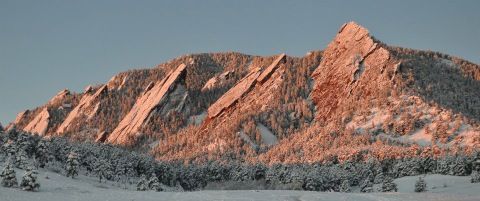
\includegraphics[scale=0.7]{./img/photo1.png}
            \caption{Photo 1}
            \label{fig:p1}
        \end{subfigure}
        \begin{subfigure}{\textwidth}
            \centering
            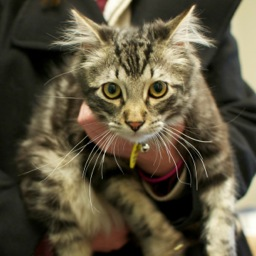
\includegraphics[scale=0.7]{./img/photo2.png}
            \caption{Photo 2}
            \label{fig:p2}
        \end{subfigure}
        \caption{Provided Images}
        \label{fig:init_image}
    \end{figure}

\section{Reading Image Files \& Grayscale Conversion}

Colored images have an interesting, although problematic property; they do not readily lend themselves to matrix manipulation because in order to get color images, seperate values are used to represent each primary color, which are then mixed together for the final color.  For example, in Figure~\ref{fig:example}, the block represents very simple a 2$\times$2 pixel image.

    \begin{figure}[ht]
        \centering
        
\includegraphics[scale=40]{./img/sqr.png}
        \caption{A simple RGB image}
        \label{fig:example}
    \end{figure}

This very simple image can be represented as either a trio of primary color matrices where each entry in each primary color matrix coresponds to the same pixel:

    \[
    \underbrace{
    \begin{bmatrix}
        1&0\\
        0&1\\
    \end{bmatrix}
    }_{\text{Red Matrix}}
    ,
    \underbrace{
    \begin{bmatrix}
        0&0\\
        1&1\\
    \end{bmatrix}
    }_{\text{Blue Matrix}}
    ,
    \underbrace{
    \begin{bmatrix}
        0&1\\
        0&0\\
    \end{bmatrix}
    }_{\text{Green Matrix}}
    \]

A single matrix may be used, with each entry being a submatrix, wherein each element in the submatrix corresponds to a primary color.

  \[
    \begin{bmatrix}
        \begin{bmatrix}1\\0\\0\end{bmatrix} &
        \begin{bmatrix}0\\1\\0\end{bmatrix}\\[2em]
        \begin{bmatrix}0\\0\\1\end{bmatrix} &
        \begin{bmatrix}1\\0\\1\end{bmatrix}
    \end{bmatrix}
  \]

Using one of the given images, the splitting of color channels gives the following set of images shown in Figure~\ref{3color}.

    \begin{figure}[ht]
        \centering
        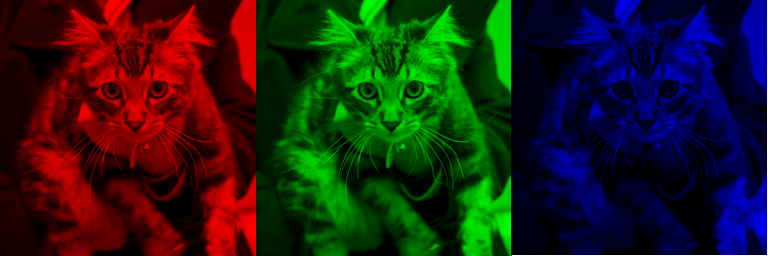
\includegraphics[scale=0.6]{./img/photo2-exploded.png}
        \caption{A given image split into its three primary color channels}
        \label{3color}
    \end{figure}

While it is possible to manipulate color images, it would be far simpler to manipulate \emph{grayscale} images, where only the final intensity is concerned. To do this, each color is considered independently for its intensity alone as shown in Figure~\ref{3gray}, where it may be scaled, and then added together to produce a final black-and-white image, which is a matrix where each entry is a single value. Note how the third panel representing the blue color channel is darker -- this implies that blue is a less intense color in the image.

    \begin{figure}[ht]
        \centering
        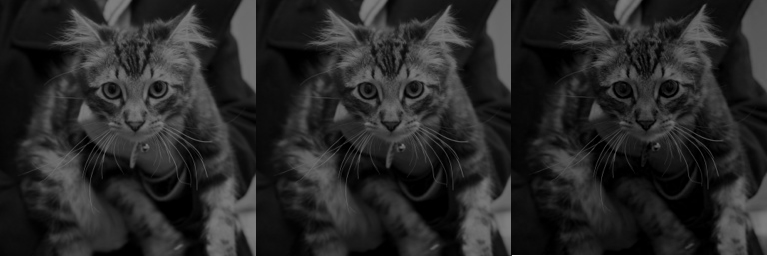
\includegraphics[scale=0.6]{./img/photo2-explodedg.png}
        \caption{A given image split into its three primary color channels, but
        only intensity of each color is shown.}
        \label{3gray}
    \end{figure}

Since each primary color is freely editable, it is simple to scale the intensity of each before mixing; in our report, we used 30\% of the red channel, 59\% of the green channel and 11\% of the blue channel. The final outputs for both given images can be seen in Figure~\ref{fig:gray_images}. Note how the final output is lighter than any of the individual color channels.

    \begin{figure}[ht]
        \centering
        \begin{subfigure}{\textwidth}
            \centering
            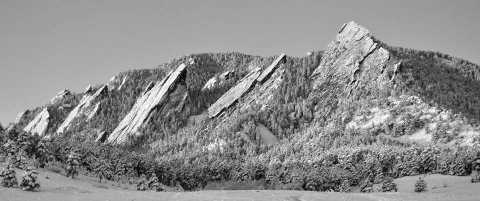
\includegraphics[scale=0.7]{./img/gray1.png}
            \caption{Photo 1 - Grayscale}
            \label{fig:p1g}
        \end{subfigure}
        \begin{subfigure}{\textwidth}
            \centering
            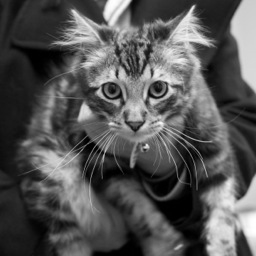
\includegraphics[scale=0.7]{./img/gray2.png}
            \caption{Photo 2 - Grayscale}
            \label{fig:p2g}
        \end{subfigure}
        \caption{Grayscale Images}
        \label{fig:gray_images}
    \end{figure}

\section{Horizontal Shifting}

Now that we are working in grayscale, it is far more straightforward to manipulate aspects of the image, such as its horizontal position.  Since we are dealing with a normal matrix, transforming the positions of columns requires only that we multiply the image matrix by a transformation identity matrix.

    \begin{figure}[ht]
        \centering
        \begin{subfigure}{\textwidth}
            \centering
            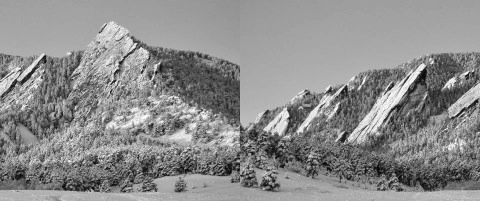
\includegraphics[scale=0.7]{./img/hsg1.png}
            \caption{Photo 1 Horizontal Shift}
            \label{fig:p1hg}
        \end{subfigure}
        \begin{subfigure}{\textwidth}
            \centering
            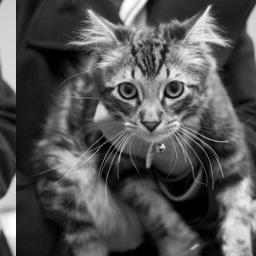
\includegraphics[scale=0.7]{./img/hsg2.png}
            \caption{Photo 2 - Horizontal Shift}
            \label{fig:p2hg}
        \end{subfigure}
        \caption{Horizontally Shifted Images}
        \label{fig:hs_images}
    \end{figure}

\section{Vertical Shifting}

\begin{figure}[ht]
    \centering
    \begin{subfigure}{\textwidth}
        \centering
        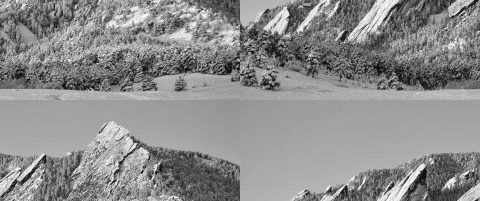
\includegraphics[scale=0.7]{./img/vhsg1.png}
        \caption{Photo 1 - Vertical and Horizontal Shift}
        \label{fig:p1vg}
    \end{subfigure}
    \begin{subfigure}{\textwidth}
        \centering
        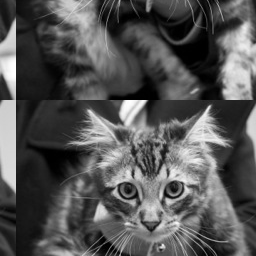
\includegraphics[scale=0.7]{./img/vhsg2.png}
        \caption{Photo 2 - Vertital and Horizontal Shift}
        \label{fig:p2vg}
    \end{subfigure}
    \caption{Vertically Shifted Images}
    \label{fig:vs_images}
\end{figure}

\newpage

\section{Inversion}

\section{Transposition}

\section{Discrete Sine Transform}

\section{DST Restrictions}

\section{Reversing the DST}

\section{Compression}

\section{Optimization}

\newpage

\appendix

\section{Code}

The entire codebase for the project follows, and is available for download \attachfile{./code.tar.gz}{here}\footnote{If you are unable to download the code from this link, please download it from \framebox{\href{http://will-farmer.com/diffeq/Project_2_matrices/code.tar.gz}{here}}}.

    \subsection{Python}

    The Python code to generate the images is included below.

        \subsubsection{Grayscale}
        \lstinputlisting[language=Python,
                        showstringspaces=false,
                        firstline=128,
                        lastline=135,
                        frame=single,
                        basicstyle=\ttfamily,
                        keywordstyle=\color{blue},
                        numbers=left,
                        commentstyle=\color{red}]{./py/analysis.py}

        \subsubsection{Horizontal Shift}
        \lstinputlisting[language=Python,
                        showstringspaces=false,
                        firstline=100,
                        lastline=112,
                        frame=single,
                        basicstyle=\ttfamily,
                        keywordstyle=\color{blue},
                        numbers=left,
                        commentstyle=\color{red}]{./py/analysis.py}

        \subsubsection{Vertical Shift}
        \lstinputlisting[language=Python,
                        showstringspaces=false,
                        firstline=114,
                        lastline=126,
                        frame=single,
                        basicstyle=\ttfamily,
                        keywordstyle=\color{blue},
                        numbers=left,
                        commentstyle=\color{red}]{./py/analysis.py}

        \subsubsection{Inversion}
        \lstinputlisting[language=Python,
                        showstringspaces=false,
                        firstline=88,
                        lastline=98,
                        frame=single,
                        basicstyle=\ttfamily,
                        keywordstyle=\color{blue},
                        numbers=left,
                        commentstyle=\color{red}]{./py/analysis.py}

        \subsubsection{Discrete Sine Transform}
        \lstinputlisting[language=Python,
                        showstringspaces=false,
                        firstline=181,
                        lastline=198,
                        frame=single,
                        basicstyle=\ttfamily,
                        keywordstyle=\color{blue},
                        numbers=left,
                        commentstyle=\color{red}]{./py/analysis.py}

        \subsubsection{Compression}
        \lstinputlisting[language=Python,
                        showstringspaces=false,
                        firstline=155,
                        lastline=179,
                        frame=single,
                        basicstyle=\ttfamily,
                        keywordstyle=\color{blue},
                        numbers=left,
                        commentstyle=\color{red}]{./py/analysis.py}

        \subsubsection{Optimization}
        \lstinputlisting[language=Python,
                        showstringspaces=false,
                        firstline=216,
                        lastline=283,
                        frame=single,
                        basicstyle=\ttfamily,
                        keywordstyle=\color{blue},
                        numbers=left,
                        commentstyle=\color{red}]{./py/analysis.py}

    \newpage

    \subsection{MATLAB Code}

    Some MATLAB Code was also made that features equivalent functionality

        \subsubsection{Grayscale}

        \lstinputlisting[language=Matlab,
                        basicstyle=\ttfamily,
                        frame=single,
                        keywordstyle=\color{orange},
                        numbers=left,
                        commentstyle=\color{cyan}]{./mat2/grayscale.m}

        \subsubsection{Horizontal Shifting}

        \lstinputlisting[language=Matlab,
                        basicstyle=\ttfamily,
                        frame=single,
                        keywordstyle=\color{orange},
                        numbers=left,
                        commentstyle=\color{cyan}]{./mat2/hshift.m}

        \subsubsection{Vertical Shifting}

        \lstinputlisting[language=Matlab,
                        basicstyle=\ttfamily,
                        frame=single,
                        keywordstyle=\color{orange},
                        numbers=left,
                        commentstyle=\color{cyan}]{./mat2/vshift.m}

\end{document}
